\chapter{Parameter Estimation} \label{cha:parameterEstimation}
A central part in modelling is parameter estimation and it's often underestimated. If the parameters in the model isn't well estimated several problems arise when trying to synthesise model-based controllers. If a systems dynamics are completely unknown, a black box method is used \textit{i.e.} general equations are fitted to test data. When a system can be completely modelled analytically for example via Newtons laws its called white box modelling. In our case the model of the system is known but several parameters are unknown, that is called gray box modelling. 

\todo{Write about kinetics in \Chapterref{cha:modelling}}

To estimate the unknown parameters in the \abbrROV model described in \Chapterref{cha:modelling} different methods can be used. Relations between states can be used to get better estimates of parameters for example if the angles of the \abbrROV are estimated well the relations
\begin{align}
\pdot &= \rollVelocity + \pitchVelocity \sin \rollAngle \tan \pitchAngle + \yawVelocity \cos \rollAngle \tan \pitchAngle,\\
\qdot &= \pitchVelocity \cos \rollAngle - \yawVelocity \sin \rollAngle \\
&\textrm{and} \nonumber \\
\rdot &= \pitchVelocity \frac{\sin \rollAngle}{\cos \pitchAngle} + \rollVelocity \frac{\cos \rollAngle}{\cos \pitchAngle}
\end{align}
from \Chapterref{cha:modelling} could be used. Another aspect to consider when estimating model parameters is what to use as inputs and outputs. Inputs to a system is considered to be true signals, thus if they are noisy or inaccurate it can effect the estimation negatively. Outputs from a system are measurements, thus are they considered to be somewhat uncertain. The attitude model structure from \Chapterref{cha:modelling} is reduced to 
\begin{multline} \label{eq:p_dotWithoutTranslation}
\dot{p} = \frac{\thrusterfun{1} \distance{y}{1} - \thrusterfun{2} \distance{y}{2} + \thrusterfun{6} \distance{z}{6}}{\Ix - \Kpdot} + \frac{p (Kp + \Kpabsp \abs{p})}{\Ix - \Kpdot} + \frac{-\Mqdot q r}{\Ix - \Kpdot} + \frac{\Nrdot q r}{\Ix - \Kpdot} +\\
\frac{q r (\Iy - \Iz)}{\Ix - \Kpdot} + \frac{B \cos{\theta} \sin{\phi} z_B}{\Ix - \Kpdot},
\end{multline} 
\begin{multline} \label{eq:q_dotWithoutTranslation}
\dot{q} =\frac{\thrusterfun{1} \distance{x}{1} + \thrusterfun{2} \distance{x}{2} - \thrusterfun{5} \distance{x}{5}}{\Iy - \Mqdot} + \frac{q (\Mq + \Mqabsq \abs{q})}{\Iy - \Mqdot} + \frac{\Kpdot p r}{\Iy - \Mqdot} + \frac{-\Nrdot p r}{\Iy - \Mqdot} +\\
\frac{p r (\Iz - \Ix)}{\Iy - \Mqdot} + \frac{B \sin{\theta} z_B}{\Iy - \Mqdot}\ \textrm{and}
\end{multline} 
\begin{multline} \label{eq:r_dotWithoutTranslation}
\dot{r} = \frac{\thrusterfun{3} \distance{y}{3} - \thrusterfun{4} \distance{y}{4}}{\Iz - \Nrdot} + \frac{r (\Nr + \Nrabsr \abs{r})}{\Iz - \Nrdot} + \frac{-\Kpdot p q}{\Iz - \Nrdot} + \frac{\Mqdot p q}{\Iz - \Nrdot} + \frac{p q (\Ix - \Iy)}{\Iz - \Nrdot}
\end{multline} 
Because the translation dynamics in the attitude model structure are assumed to be small.

%%%%%%%%%%%%%%%%%%%%%%%%%%%%%%%%%%%%%%%%%%%%%%%%%%%%%%%%%%%
\section{Parameter Estimation} 
In general parameter estimation is to fit the model structure's parametrising vector $\boldsymbol{\theta}$ to estimation data. The fitting is done by minimising the cost function $V(\boldsymbol{\theta})$ with respect to the parameter vector $\boldsymbol{\theta}$ \emph{i.e.}
\begin{equation}
\hat{\boldsymbol{\theta}} = \underset{\boldsymbol{\theta}}{\argmin} V(\boldsymbol{\theta})
\end{equation}
The cost function in this thesis has been defined as the squared error
\begin{equation}
    V(\boldsymbol{\theta}) = \frac{1}{N} \sum_{t=1}^{N} e^T(t,\boldsymbol{\theta}) W(\boldsymbol{\theta})  e(t,\boldsymbol{\theta})
\end{equation}
where:
\begin{itemize}
    \item $N$ is the number of samples.
    \item $e(t,\boldsymbol{\theta}) = y(t) - \hat{y}(t|\boldsymbol{\theta})$ is the error vector at time t with the parameter vector~$\boldsymbol{\theta}$.
    \item $W(\boldsymbol{\theta})$ is the positive definite weight matrix.
\end{itemize}

A general model structure can be described by
\begin{equation}
\dot{x}(t) = f(x(t), u(t), \boldsymbol{\theta})
\end{equation}
and
\begin{equation}
\hat{y}(t|\boldsymbol{\theta}) = h(x(t), u(t), \boldsymbol{\theta})
\end{equation}
 where:
 \begin{itemize}
  \item $\hat{y}(t|\boldsymbol{\theta})$ is the predicted output.
  \item $x(t)$ are the states. 
  \item $u(t)$ are the inputs. 
 \end{itemize}
A measure of how well the model describes the data can be
\begin{equation}
Fit = 100 \Biggr(1 - \frac{\sqrt{\sum\limits_{t=1}^N (y(k) - \hat{y}(t))^2}}{\sqrt{\sum\limits_{t=1}^N(y(t)-\frac{1}{N}\sum\limits_{t=1}^N y(t))^2}}\Biggl)
\end{equation} 
Higher percentage often indicate that the model describes the data well. 
%%%%%%%%%%%%%%%%%%%%%%%%%%%%%%%%%%%%%%%%%%%%%%%%%%%%%%%%%%%
\section{Decoupling the Model}
The attitude model structure of the \abbrROV was divided into three estimation steps. From \eqref{eq:p_dot} - \eqref{eq:r_dot} it can be seen that $\rdot$ aren't effected by the same thrusters as $\pdot$ and $\qdot$. Thus was the yaw models parameters initially estimated by themselves and the roll and pitch models parameters estimated by themselves. The initially estimated parameters was then used in the complete attitude model parameter estimation, \eqref{eq:p_dotWithoutTranslation} - \eqref{eq:r_dotWithoutTranslation}. The initial models for yaw and roll and pitch dynamics that was used was the reduced model structure
\begin{align} \label{eq:pq_dot_simple}
\dot{p} &= \frac{\thrusterfun{1} \distance{y}{1} - \thrusterfun{2} \distance{y}{2} + \thrusterfun{6} \distance{z}{6}}{\Ix - \Kpdot} + \frac{p (Kp + \Kpabsp \abs{p})}{\Ix - \Kpdot} + \frac{B \cos{\theta} \sin{\phi} z_B}{\Ix - \Kpdot}, \\ \label{eq:pq_dot_simple2}
\dot{q} &=\frac{\thrusterfun{1} \distance{x}{1} + \thrusterfun{2} \distance{x}{2} - \thrusterfun{5} \distance{x}{5}}{\Iy - \Mqdot} + \frac{q (\Mq + \Mqabsq \abs{q})}{\Iy - \Mqdot} + \frac{B \sin{\theta} z_B}{\Iy - \Mqdot} 
\end{align} and
\begin{equation} \label{eq:r_dot_simple}
\dot{r} = \frac{\thrusterfun{3} \distance{y}{3} - \thrusterfun{4} \distance{y}{4}}{\Iz - \Nrdot} + \frac{r (\Nr + \Nrabsr \abs{r})}{\Iz - \Nrdot}
\end{equation}
This could be done because the tests only excited the states used in that estimation and thus was the coupled terms assumed to be zero.

%%%%%%%%%%%%%%%%%%%%%%%%%%%%%%%%%%%%%%%%%%%%%%%%%%%%%%%%%%%
\section{Data Collection}
The main test signals used in the parameter estimation tests was telegraph signals. Both the scaling of the output signals and switch factors was changed in between tests for finding signals that excited the \abbrROV sufficiently.
Three different tests was conducted 
\begin{description}
\item[Yaw test] Telegraph signals on thrusters 3 and 4 was used for exciting the \abbrROV in \yawAngle-direction.
\item[Roll and pitch test] Telegraph signals on thrusters 1, 2, 5 and 6 was used for exciting the \abbrROV in \rollAngle- and \pitchAngle-direction.
\item[Complete test] Telegraph signals on all the thrusters used for exciting the \abbrROV about every axis.
\end{description}

%%%%%%%%%%%%%%%%%%%%%%%%%%%%%%%%%%%%%%%%%%%%%%%%%%%%%%%%%%%
\section{Parameter Estimation from Angular Velocities}
Due to poorly estimated angles as can be seen in \Figureref{fig:integratedAngleVelocities}, the angles was not suited to be used in the parameter estimation. Thus was the parameters estimated using the angular velocities as measurements. This method was used when the sensor fusion algorithms described in \Sectionref{sec:angularVelocityKalman} was used.

\begin{figure}[tbp]
  \centering
  \subfloat[][\label{fig:velocityAnglePhi}A comparison of integration of angular velocities transformed to the global frame (blue) against the estimated angel \rollAngle (red).]{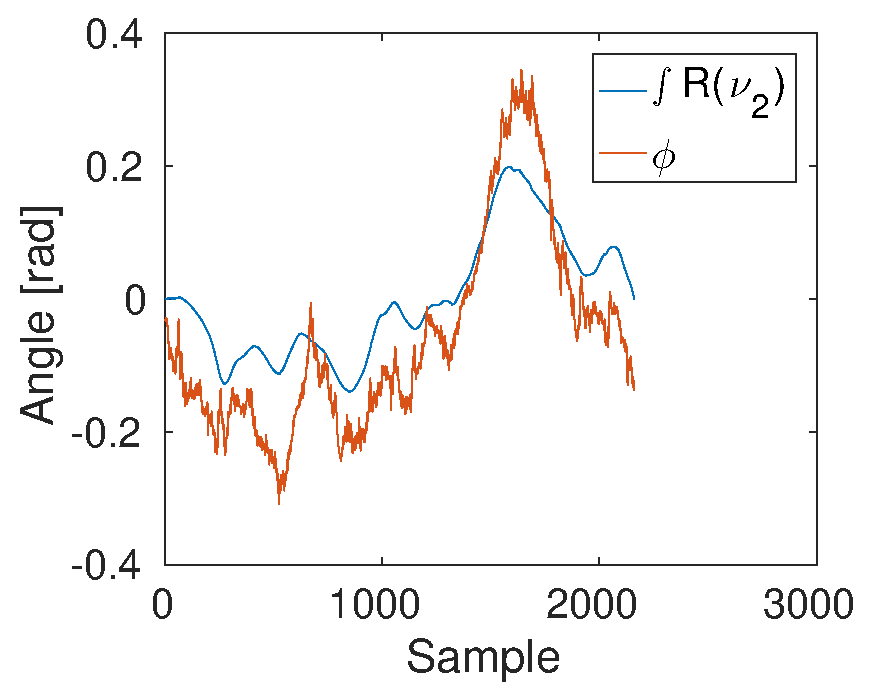
\includegraphics[width=0.5\textwidth]{velocityAnglePhi}}
  \qquad
  \subfloat[][\label{fig:velocityAngleTheta}A comparison of integration of angular velocities transformed to the global frame (blue) against the estimated angel \pitchAngle (red).]{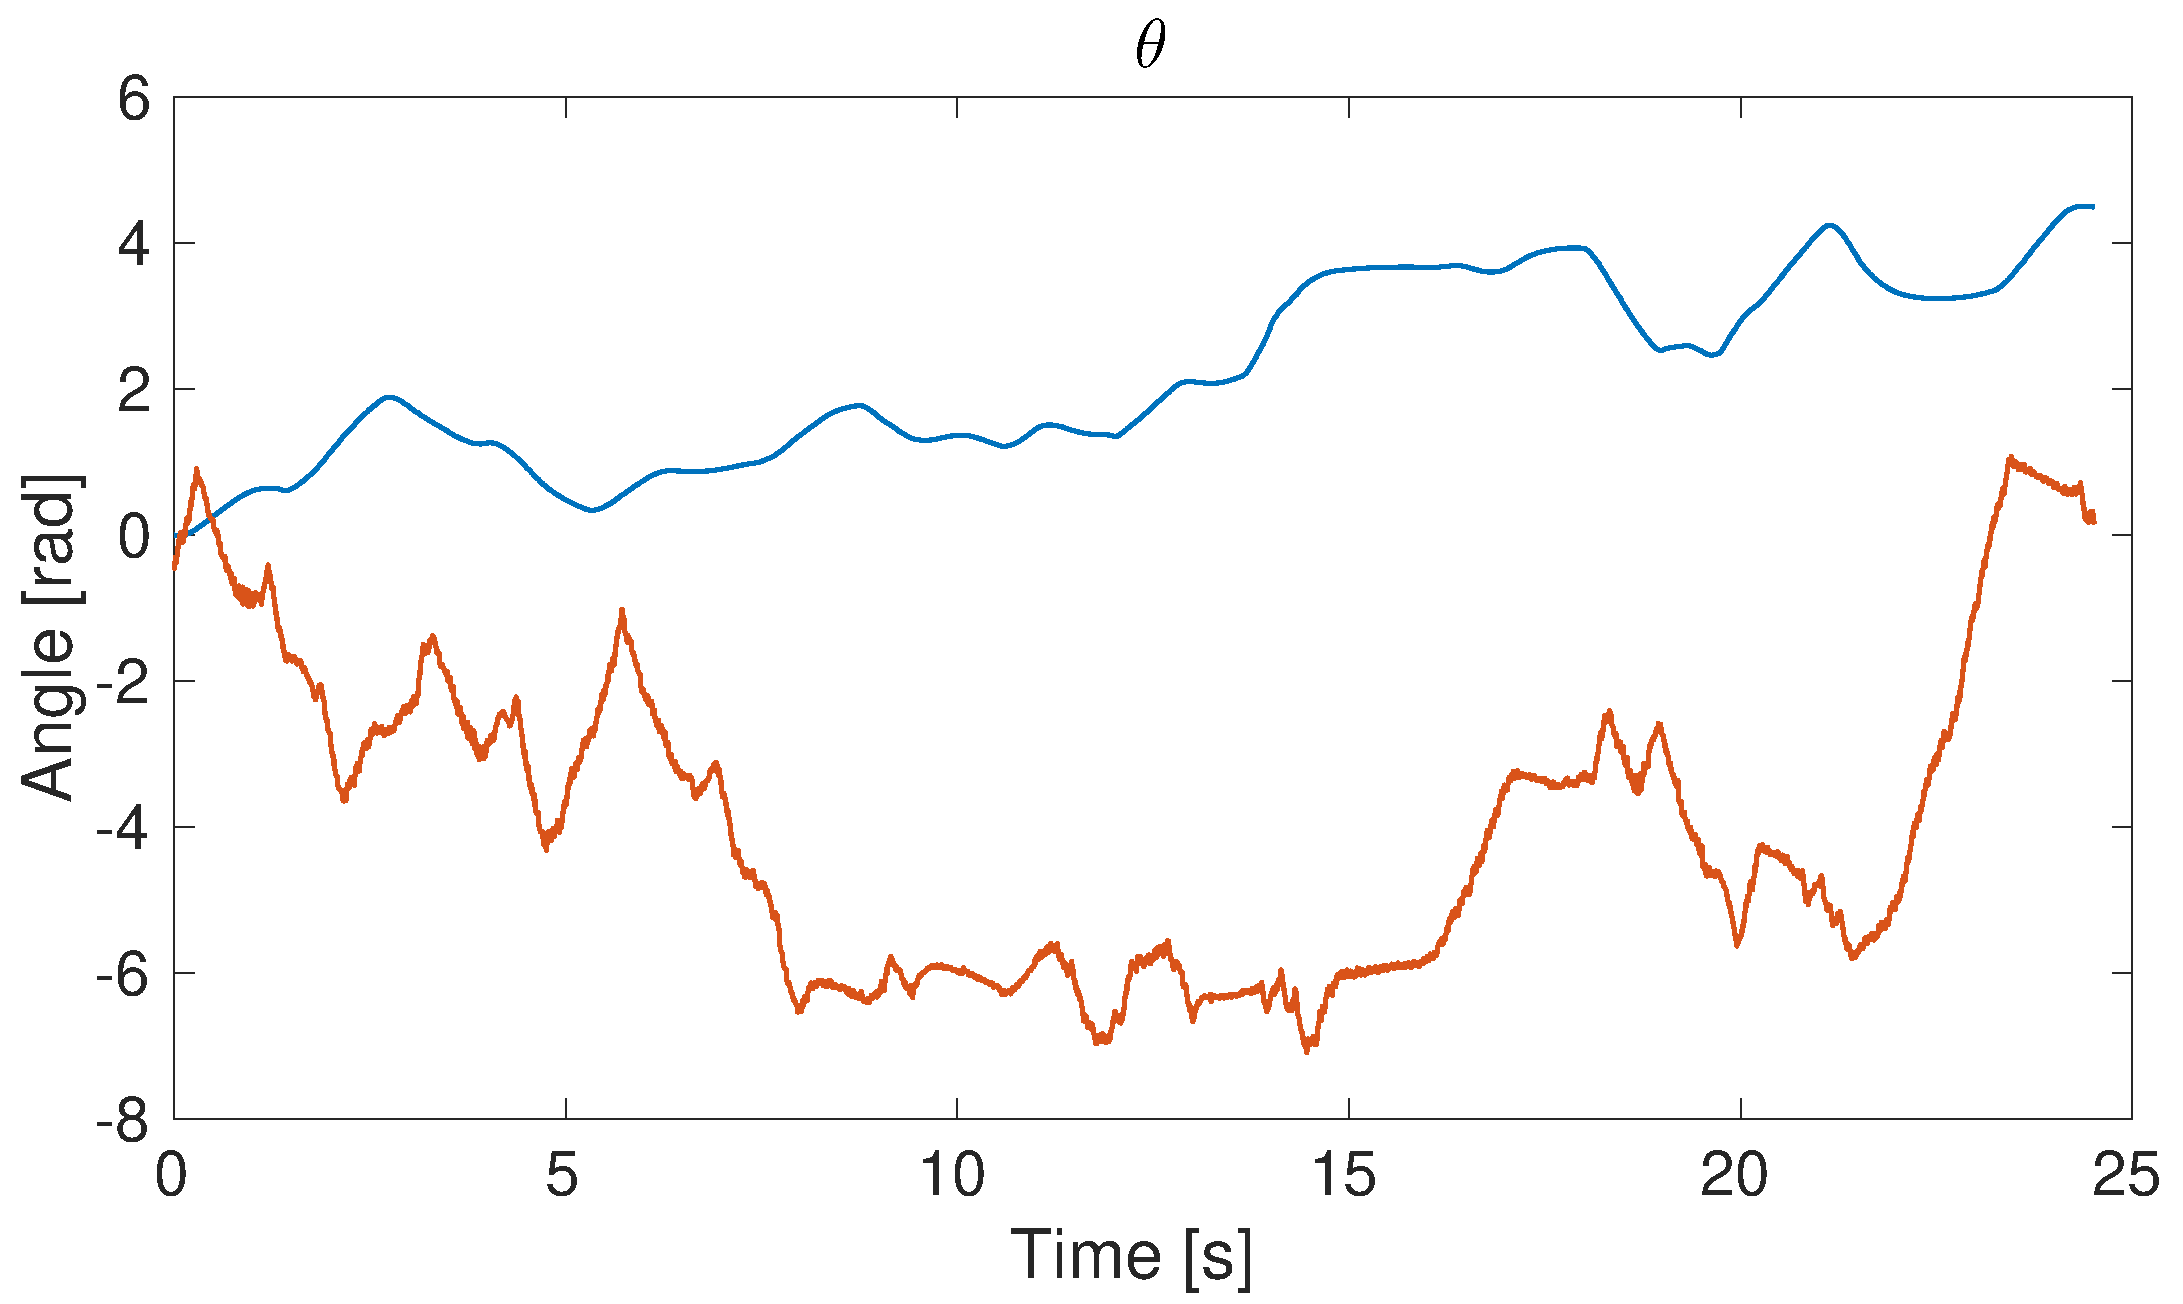
\includegraphics[width=0.5\textwidth]{velocityAngleTheta}}
  \\
  \subfloat[][\label{fig:velocityAnglePsi}A comparison of integration of angular velocities transformed to the global frame (blue) against the estimated angel \yawAngle (red).]{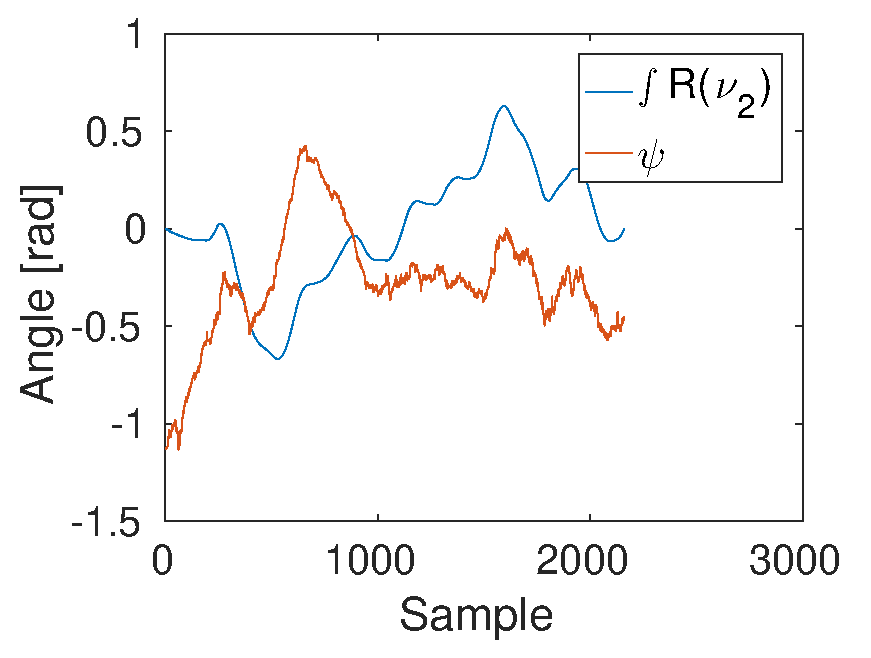
\includegraphics[width=0.5\textwidth]{velocityAnglePsi}}
  \caption{\label{fig:integratedAngleVelocities}%
    As can be seen in \protect\subref{fig:velocityAnglePhi}-\protect\subref{fig:velocityAnglePsi} the angles are poorly estimated and thus not suitable to use in parameter estimation. The angles are estimated with the method used in \Sectionref{sec:angularVelocityKalman}.}
\end{figure}

To get an initial estimate on the parameters in the yaw dynamics the reduced model parameters in \eqref{eq:r_dot_simple}
was estimated. The estimation was done with data collected from a test that mainly excited the \abbrROV in \yawAngle-direction and thus could the cross-terms be assumed to be zero.

The roll and pitch dynamics are coupled thus was \eqref{eq:pq_dot_simple} and \eqref{eq:pq_dot_simple2} estimated at the same time.
The cross terms could be assumed to be zero due to the \abbrROV was mainly excited in \rollAngle-direction and \pitchAngle-direction in the used estimation data.

The estimate of the parameters in \eqref{eq:r_dot_simple} and \eqref{eq:pq_dot_simple} was used as initial estimates of the parameters in \eqref{eq:q_dotWithoutTranslation}-\eqref{eq:r_dotWithoutTranslation}. Due to observational problems the reparametrisation $A_p = \Ix - \Kpdot$, $B_q = \Iy - \Mqdot$ and $C_r = \Iz - \Nrdot$ was done. In \Figureref{fig:velocityCompare} the simulated model without reparametrisation can be seen. A improvement of the fit can be seen in \Figureref{fig:velocityCompareCong} where some parameters has been reparameterised.

\begin{figure}[tbp]
  \centering
  \subfloat[][\label{fig:velocityComparep}Comparison between a simulated model without reparametrisation and validation data in the \rollAngle-direction.]{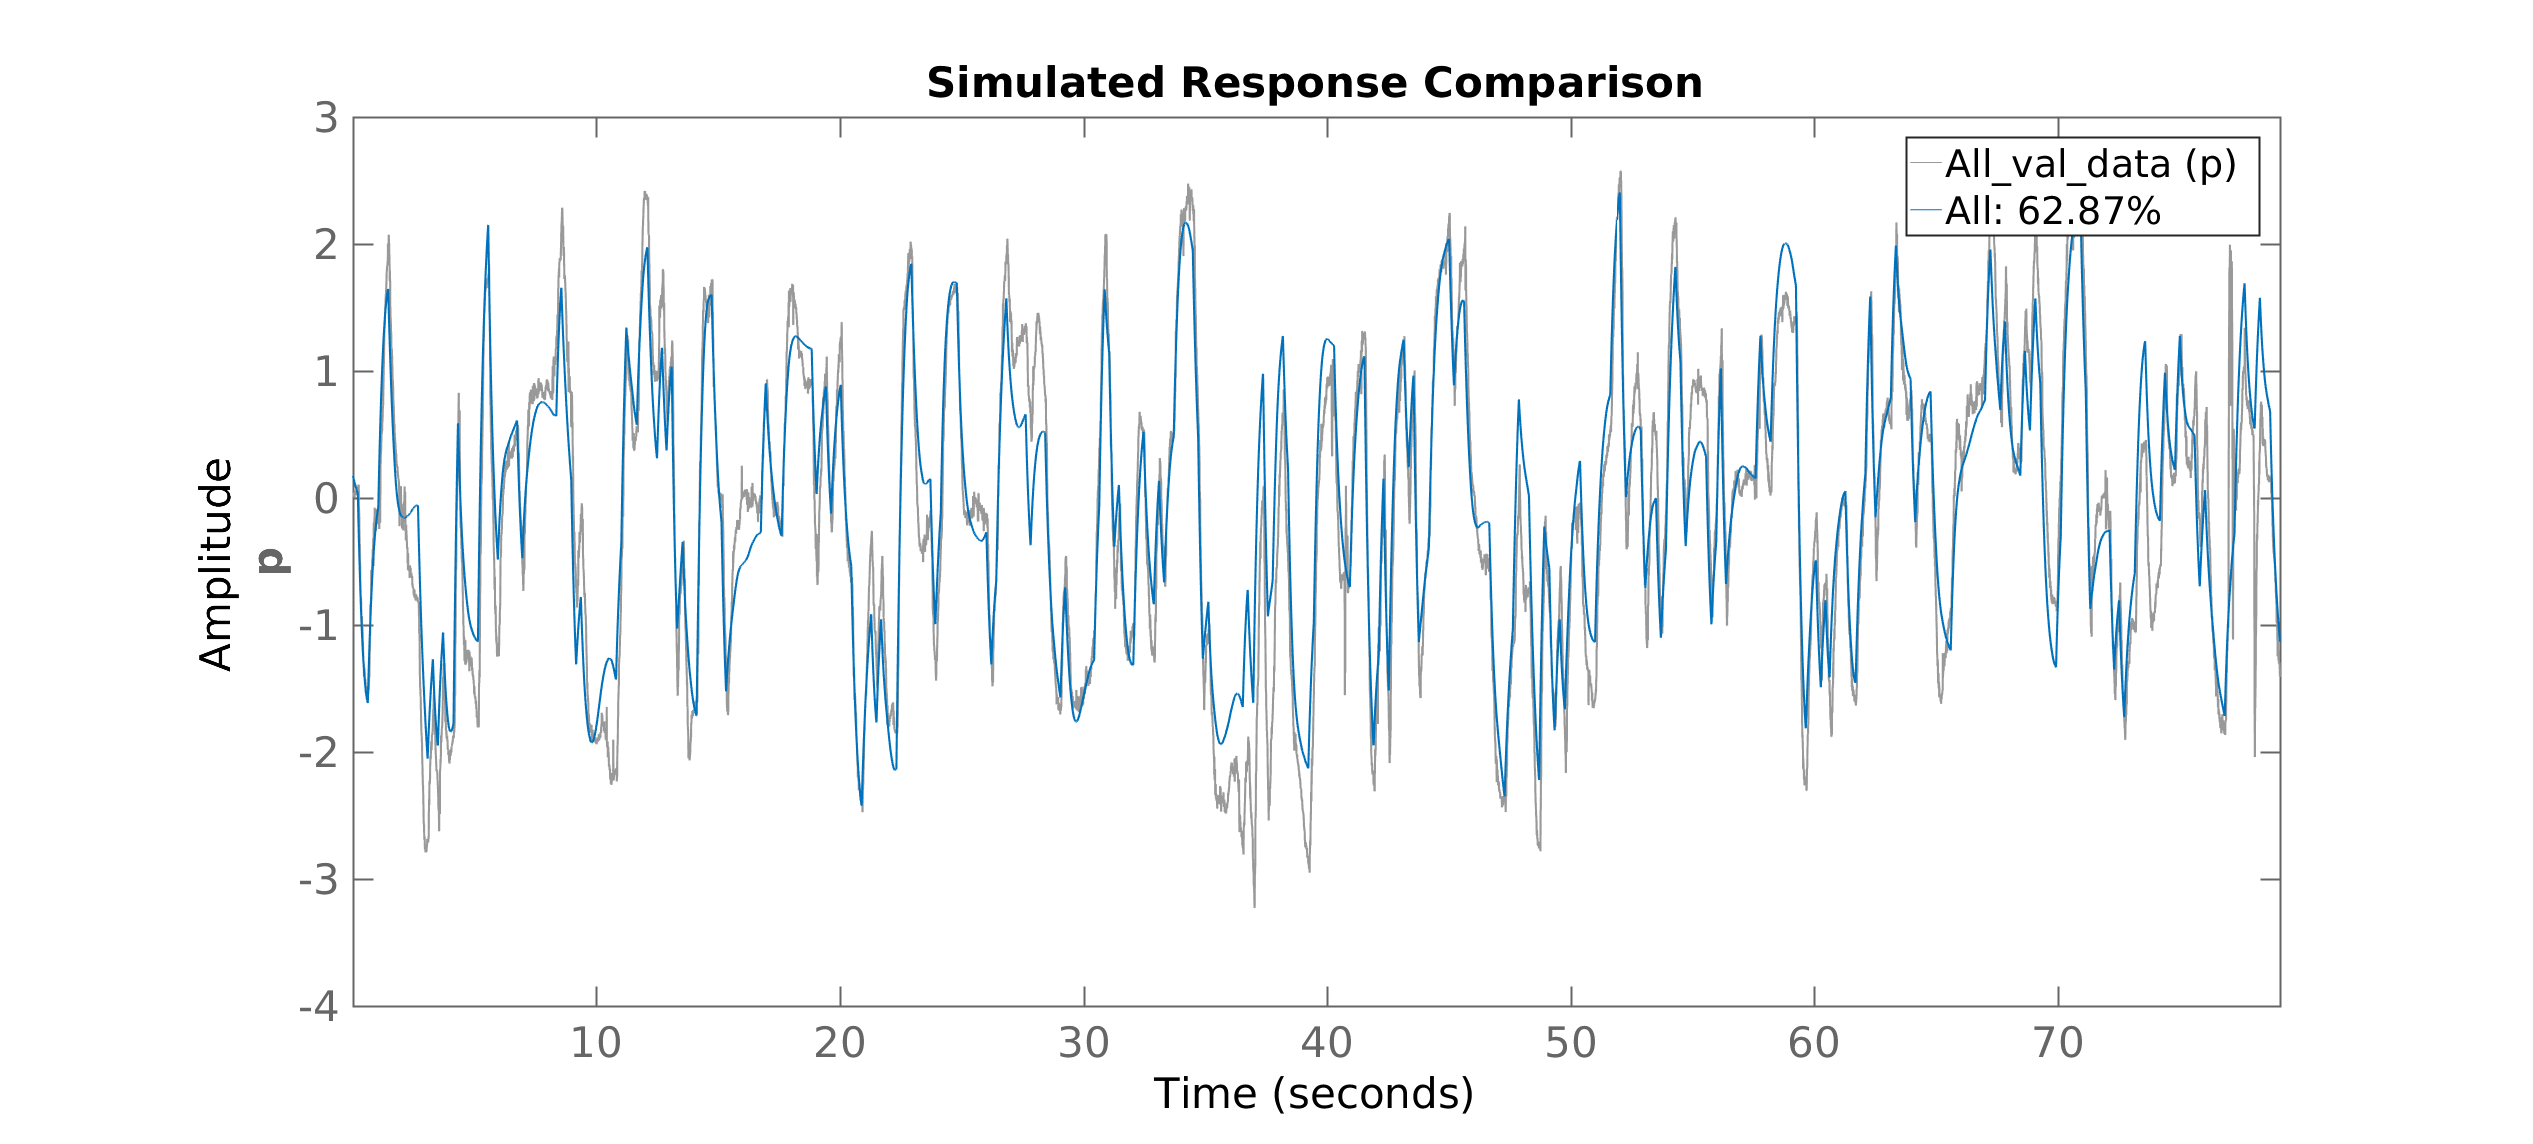
\includegraphics[width=0.8\textwidth]{velocityComparep}}
  \qquad
  \subfloat[][\label{fig:velocityCompareq}Comparison between a simulated model without reparametrisation and validation data in the \pitchAngle-direction.]{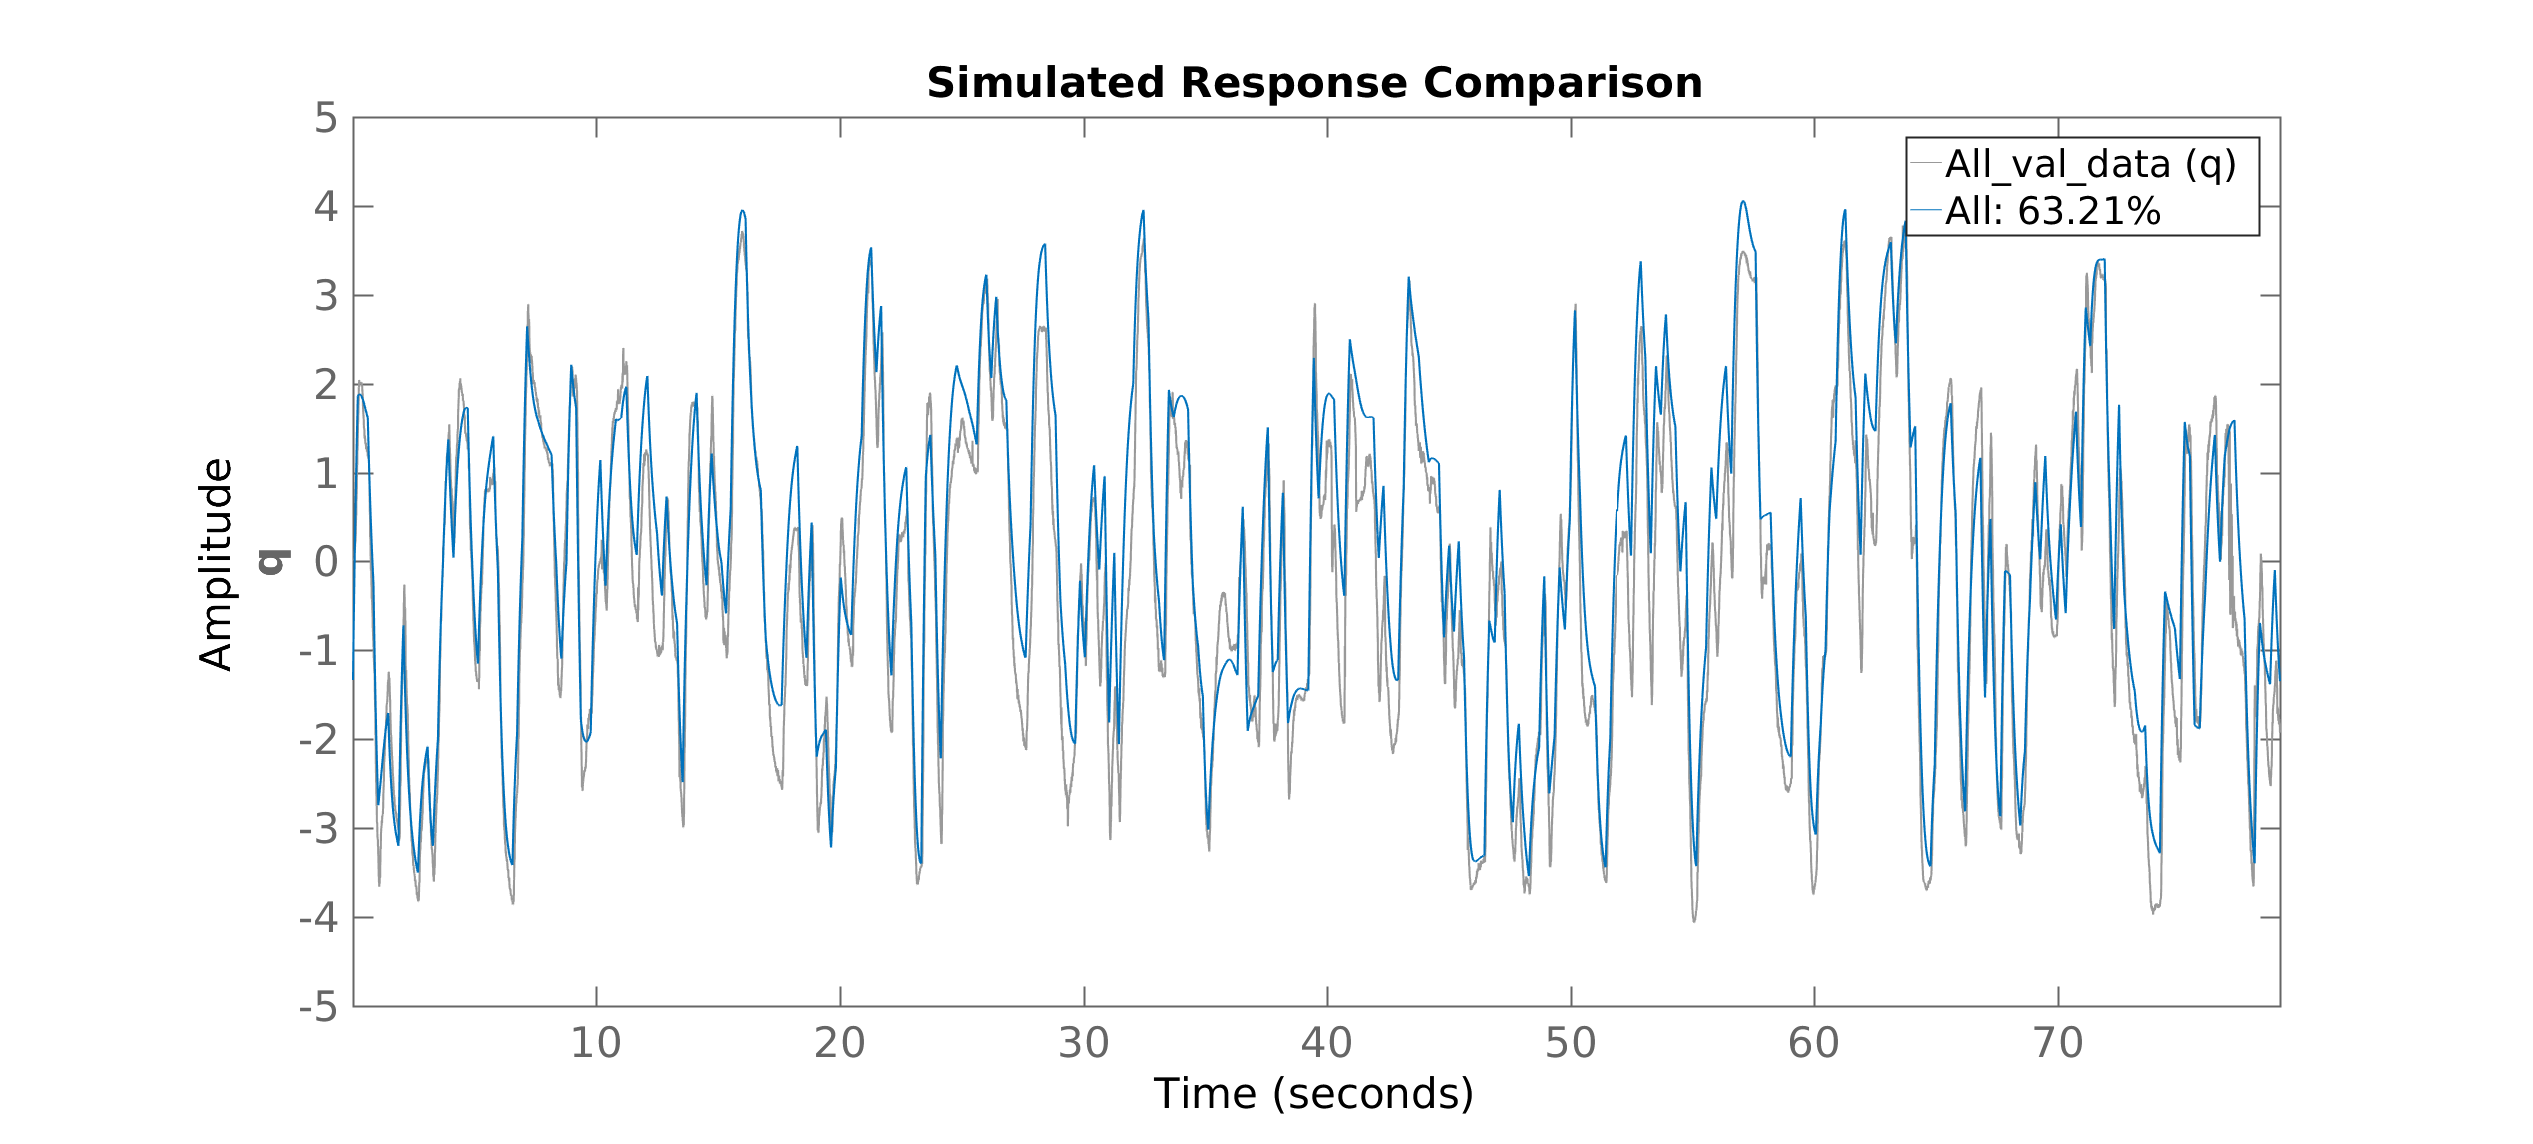
\includegraphics[width=0.8\textwidth]{velocityCompareq}}
  \\
  \subfloat[][\label{fig:velocityComparer}Comparison between a simulated model without reparametrisation and validation data in the \yawAngle-direction.]{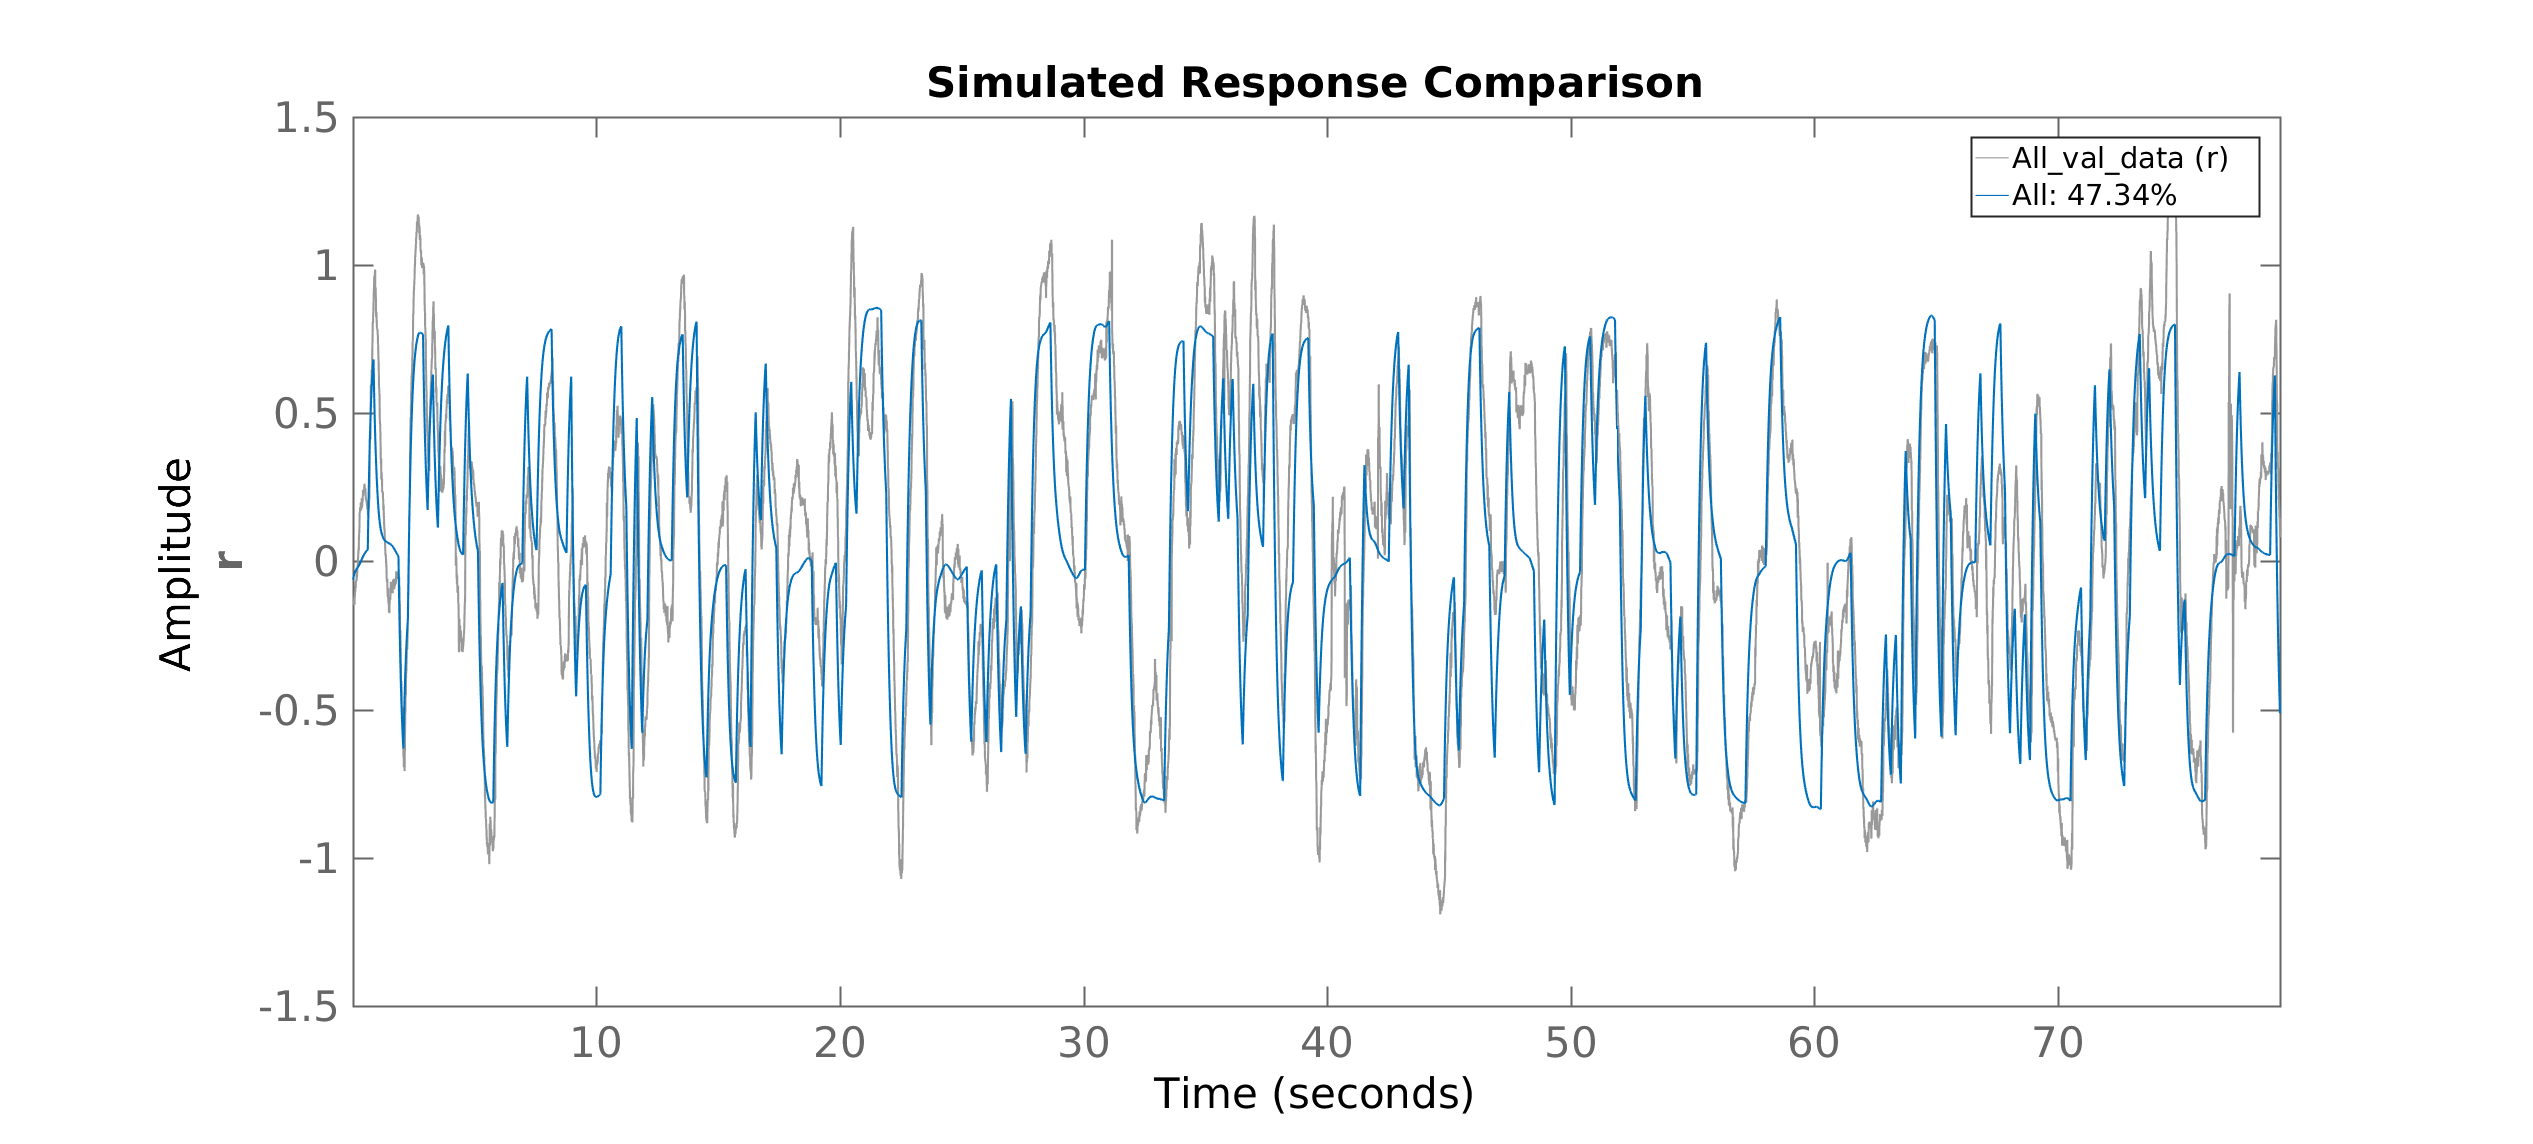
\includegraphics[width=0.8\textwidth]{velocityComparer}}
  \caption{\label{fig:velocityCompare}%
    Comparison of simulation of the attitude model against validation data.}
\end{figure}

\begin{figure}[tbp]
  \centering
  \subfloat[][\label{fig:velocityCompareCongp}Comparison between a simulated model without reparametrisation and validation data in the \rollAngle-direction.]{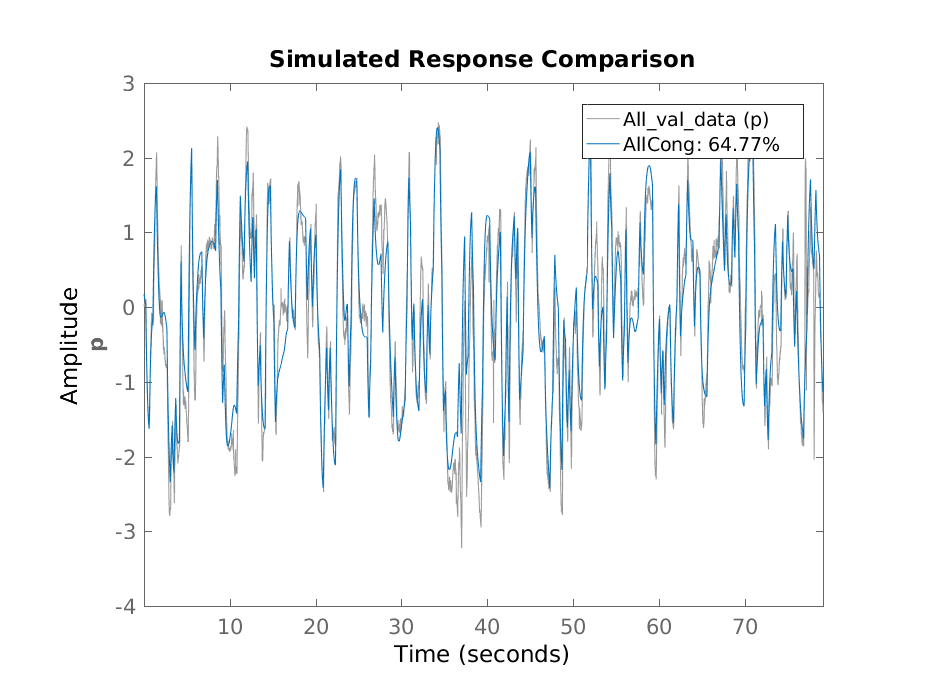
\includegraphics[width=0.5\textwidth]{velocityCompareCongp}}
  \qquad
  \subfloat[][\label{fig:velocityCompareCongq}Comparison between a simulated model without reparametrisation and validation data in the \pitchAngle-direction.]{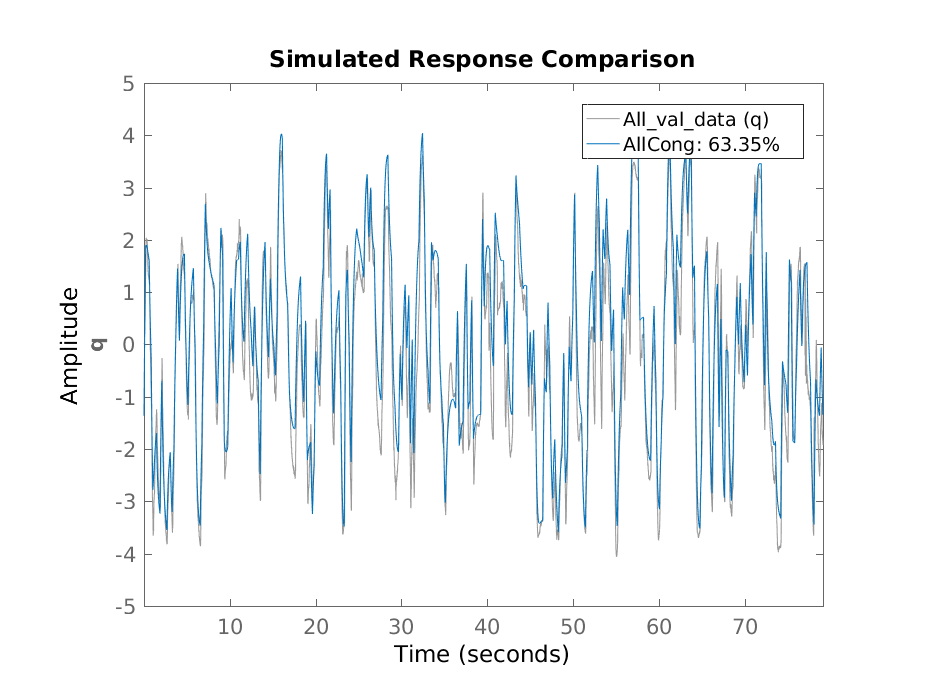
\includegraphics[width=0.5\textwidth]{velocityCompareCongq}}
  \\
  \subfloat[][\label{fig:velocityCompareCongr}Comparison between a simulated model without reparametrisation and validation data in the \yawAngle-direction.]{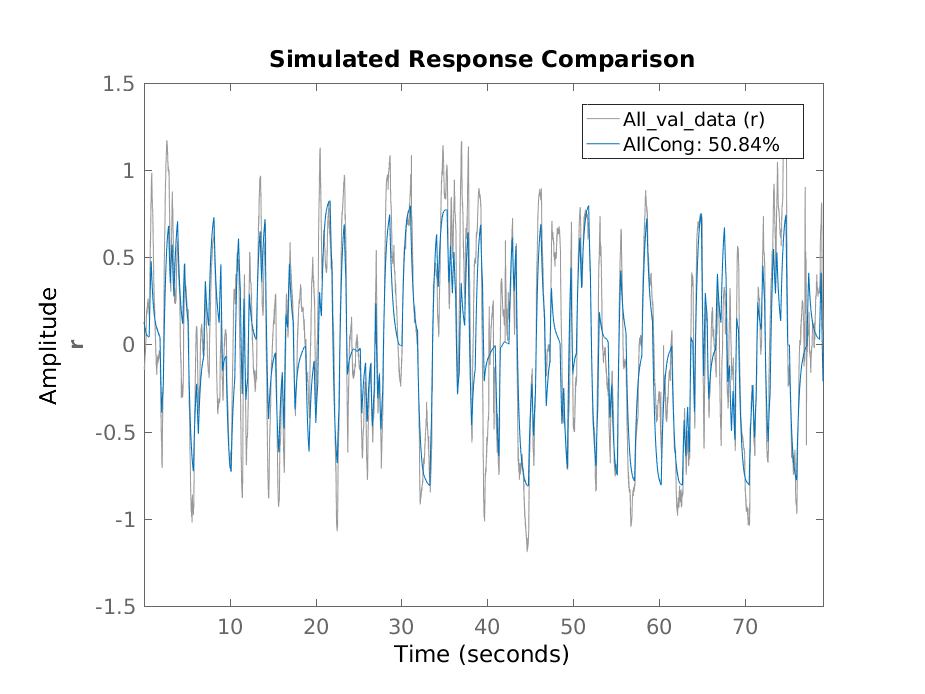
\includegraphics[width=0.5\textwidth]{velocityCompareCongr}}
  \caption{\label{fig:velocityCompareCong}%
    Comparison of simulation of the attitude model against validation data.}
\end{figure}
%%%%%%%%%%%%%%%%%%%%%%%%%%%%%%%%%%%%%%%%%%%%%%%%%%%%%%%%%%%
\subsection{Extended Kalman filter estimation}
A \abbEKF was also used to estimate parameters of the \abbROV. A congregreated model used in chapter \ref{cha:Model} was used. Each parameter was modeled as a state using a constant position model as a motion model. The complete model can be seen in equation \ref{eq:motionModelKalman}. The Kalman filter was run on each collected data set with the result of each run used as a starting state for the subsequent run.  
\begin{equation}
%insert full motion modelfor kalman estimator here.
\end{equation}




%%%%%%%%%%%%%%%%%%%%%%%%%%%%%%%%%%%%%%%%%%%%%%%%%%%%%%%%%%%
\subsection{Validation}
%%%%%%%%%%%%%%%%%%%%%%%%%%%%%%%%%%%%%%%%%%%%%%%%%%%%%%%%%%%
\section{Estimated parameters}
\Tableref{tab:parameterEstimation} shows the constants and parameters used in the \abbrROV model.

 \begin{table}[tbp]
  \centering
  \caption{\label{tab:parameterEstimation}%
    The constants and estimated parameters used in the \abbrROV model.}
\scalebox{0.85}{
  \begin{tabular}{l l p{0.7\linewidth}}
    \toprule%
    \textbf{Notation}   & \textbf{Value} & \textbf{Description} \\
    \otoprule%
    $m$                 & 6.621 \kilogram                    & Mass of the \abbrROV. \\            
    $g$                 & 9.82  \meter\per\second\squared    & Gravity acceleration.\\   
    $\rho$              & 1000  \kilogram\per\meter\cubed    & Density of water.\\ 
    $V$                 &        \meter\cubed                & Displaced volume.\\       
    
    $\distance{x}{1}$   & 0.16 \meter & Distance from \abbrCG to thruster 1 in $\xPosition$-direction.\\
    $\distance{y}{1}$   & 0.11 \meter & Distance from \abbrCG to thruster 1 in $\yPosition$-direction.\\
    $\distance{y}{2}$   & 0.11 \meter & Distance from \abbrCG to thruster 2 in $\yPosition$-direction.\\
    $\distance{x}{2}$   & 0.16 \meter & Distance from \abbrCG to thruster 2 in $\xPosition$-direction.\\
    $\distance{y}{3}$   & 0.11 \meter & Distance from \abbrCG to thruster 3 in $\yPosition$-direction.\\
    $\distance{x}{5}$   & 0.2  \meter & Distance from \abbrCG to thruster 5 in $\xPosition$-direction.\\
    $\distance{y}{4}$   & 0.11 \meter & Distance from \abbrCG to thruster 4 in $\yPosition$-direction.\\
    $\distance{z}{6}$   & 0.11 \meter & Distance from \abbrCG to thruster 6 in $\zPosition$-direction.\\
    $z_B$               &   \meter& Distance from \abbrCG to \abbrCB.\\
    
    % Parameters that will be estimated
    $\Xu$               &   \kilogram\per\second                        & Linear damping coefficient in $\xPosition$-direction due to translation in water.\\
    $\Xudot$            &   \kilogram                                   & Added mass in $\xPosition$-direction due to translation in water.\\
    $\Xuabsu$           &   \kilogram\per\meter                         & Quadratic damping coefficient in $\xPosition$-direction due to translation in water.\\
    $\Yv$               &   \kilogram\per\second                        & Linear damping coefficient in $\yPosition$-direction due to translation in water.\\
    $\Yvdot$            &   \kilogram                                   & Added mass in $\yPosition$-direction due to translation in water.\\
    $\Yvabsv$           &   \kilogram\per\meter                         & Quadratic damping coefficient in $\yPosition$-direction due to translation in water.\\
    $\Zw$               &   \kilogram\per\second                        & Linear damping coefficient in $\zPosition$-direction due to translation in water.\\
    $\Zwdot$            &   \kilogram                                   & Added mass in $\zPosition$-direction due to translation in water.\\
    $\Zwabsw$           &   \kilogram\per\meter                         & Quadratic damping coefficient in $\zPosition$-direction due to translation in water.\\
    $\Kp$               &   \kilogram\usk\meter\squared                 & Linear damping coefficient due to rotation in water about the $\xPosition$-axis.\\
    $\Kpdot$            &   \kilogram\usk\meter\squared\per\usk\second  & Increased inertia about the $\xPosition$-axis due to rotation in water.\\
    $\Kpabsp$           &   \kilogram\usk\meter\squared                 & Quadratic damping coefficient due to rotation in water about the $\xPosition$-axis.\\
    $\Mq$               &   \kilogram\usk\meter\squared                 & Linear damping coefficient due to rotation in water about the $\yPosition$-axis.\\
    $\Mqdot$            &   \kilogram\usk\meter\squared\per\usk\second  & Increased inertia about the $\yPosition$-axis due to rotation in water.\\
    $\Mqabsq$           &   \kilogram\usk\meter\squared                 & Quadratic damping coefficient due to rotation in water about the $\yPosition$-axis.\\
    $\Nr$               &   \kilogram\usk\meter\squared                 & Linear damping coefficient due to rotation in water about the $\zPosition$-axis.\\
    $\Nrdot$            &   \kilogram\usk\meter\squared\per\usk\second  & Increased inertia about the $\zPosition$-axis due to rotation in water.\\
    $\Nrabsr$           &   \kilogram\usk\meter\squared                 & Quadratic damping coefficient due to rotation in water about the $\zPosition$-axis.\\
    $\Ix$               &   \kilogram\usk\meter\squared                 & Inertia around the $\xPosition$-axis.\\
    $\Iy$               &   \kilogram\usk\meter\squared                 & Inertia around the $\yPosition$-axis.\\
    $\Iz$               &   \kilogram\usk\meter\squared                 & Inertia around the $\zPosition$-axis.\\
    \bottomrule%
  \end{tabular}}
\end{table}
%%%%%%%%%%%%%%%%%%%%%%%%%%%%%%%%%%%%%%%%%%%%%%%%%%%%%%%%%%%
\section{Parameter Estimation from Angular Velocities and Linear Acceleration}

%%%%%%%%%%%%%%%%%%%%%%%%%%%%%%%%%%%%%%%%%%%%%%%%%%%%%%%%%%%
\subsection{Validation}

%%%%%%%%%%%%%%%%%%%%%%%%%%%%%%%%%%%%%%%%%%%%%%%%%%%%%%%%%%%
\section{Estimated parameters}